\section{The constant \texorpdfstring{$A(p)$}{A(p)}}
\label{sec:Ap}

Everything in \cref{sec:qsd} reduced to the single constant
\begin{equation}
\label{eq:Ap-def}
A(p) = \lim_{n\to\infty}\frac{S_n}{(2p)^n},\qquad p\in[0,\tfrac12),
\end{equation}
whose reciprocal is the quasi-stationary mean. Approximate values are easy enough to
obtain: iterate $S_{n+1} = f(S_n)$ until $S_n$ is very nearly stationary, then form
$S_n/(2p)^n$. Repeating over a range of $p$ traces the curve of \cref{fig:dtct}, and
this works well for most of the interval. It fails as $p\to\tfrac12^-$, because the
number of generations required for $S_n$ to reach near-stationarity grows without bound.

No formula in elementary functions is known for $A(p)$, and a good deal of effort went
into looking for one. This section sets out what was found: an exact infinite product
(\cref{sec:product}); an exact series with two-sided bounds that pin $A(p)$ between the
continuous-time constant of \cref{sec:cts} and twice it (\cref{sec:Abounds}); the
near-critical asymptotic $A(p)\sim2(1-2p)$ (\cref{sec:asymptotic}); a resolution of the
discrepancy between the discrete and continuous curves (\cref{sec:compare}); an account
of the symbolic-regression searches (\cref{sec:GA}); and finally the dynamical argument
that explains why the search was doomed (\cref{sec:koenigs}). \Cref{sec:practical} draws
the practical conclusions.

\subsection{An infinite-product representation}
\label{sec:product}

Take the nonlinear map for the survival probability,
\begin{equation*}
S_{n+1} = 2pS_n - pS_n^2,\qquad S_0=1,
\end{equation*}
and substitute $S_n = 2w_n$. This gives
\begin{equation}
\label{eq:logistic}
w_{n+1} = 2p\,w_n(1-w_n) = r\,w_n(1-w_n),\qquad r = 2p,\ \ w_0 = \tfrac12 ,
\end{equation}
which is the logistic map --- the same map that exhibits the celebrated period-doubling
route to chaos as $r$ increases from $0$ to $4$ (\cref{fig:period_double}). Our
subcritical window is $r\in[0,1)$, at the extreme left of that picture, where the origin
is a globally attracting fixed point. That this innocuous corner of the logistic family
is nevertheless enough to obstruct a closed form is the substance of \cref{sec:koenigs}.

\begin{figure}[ht]
    \centering
    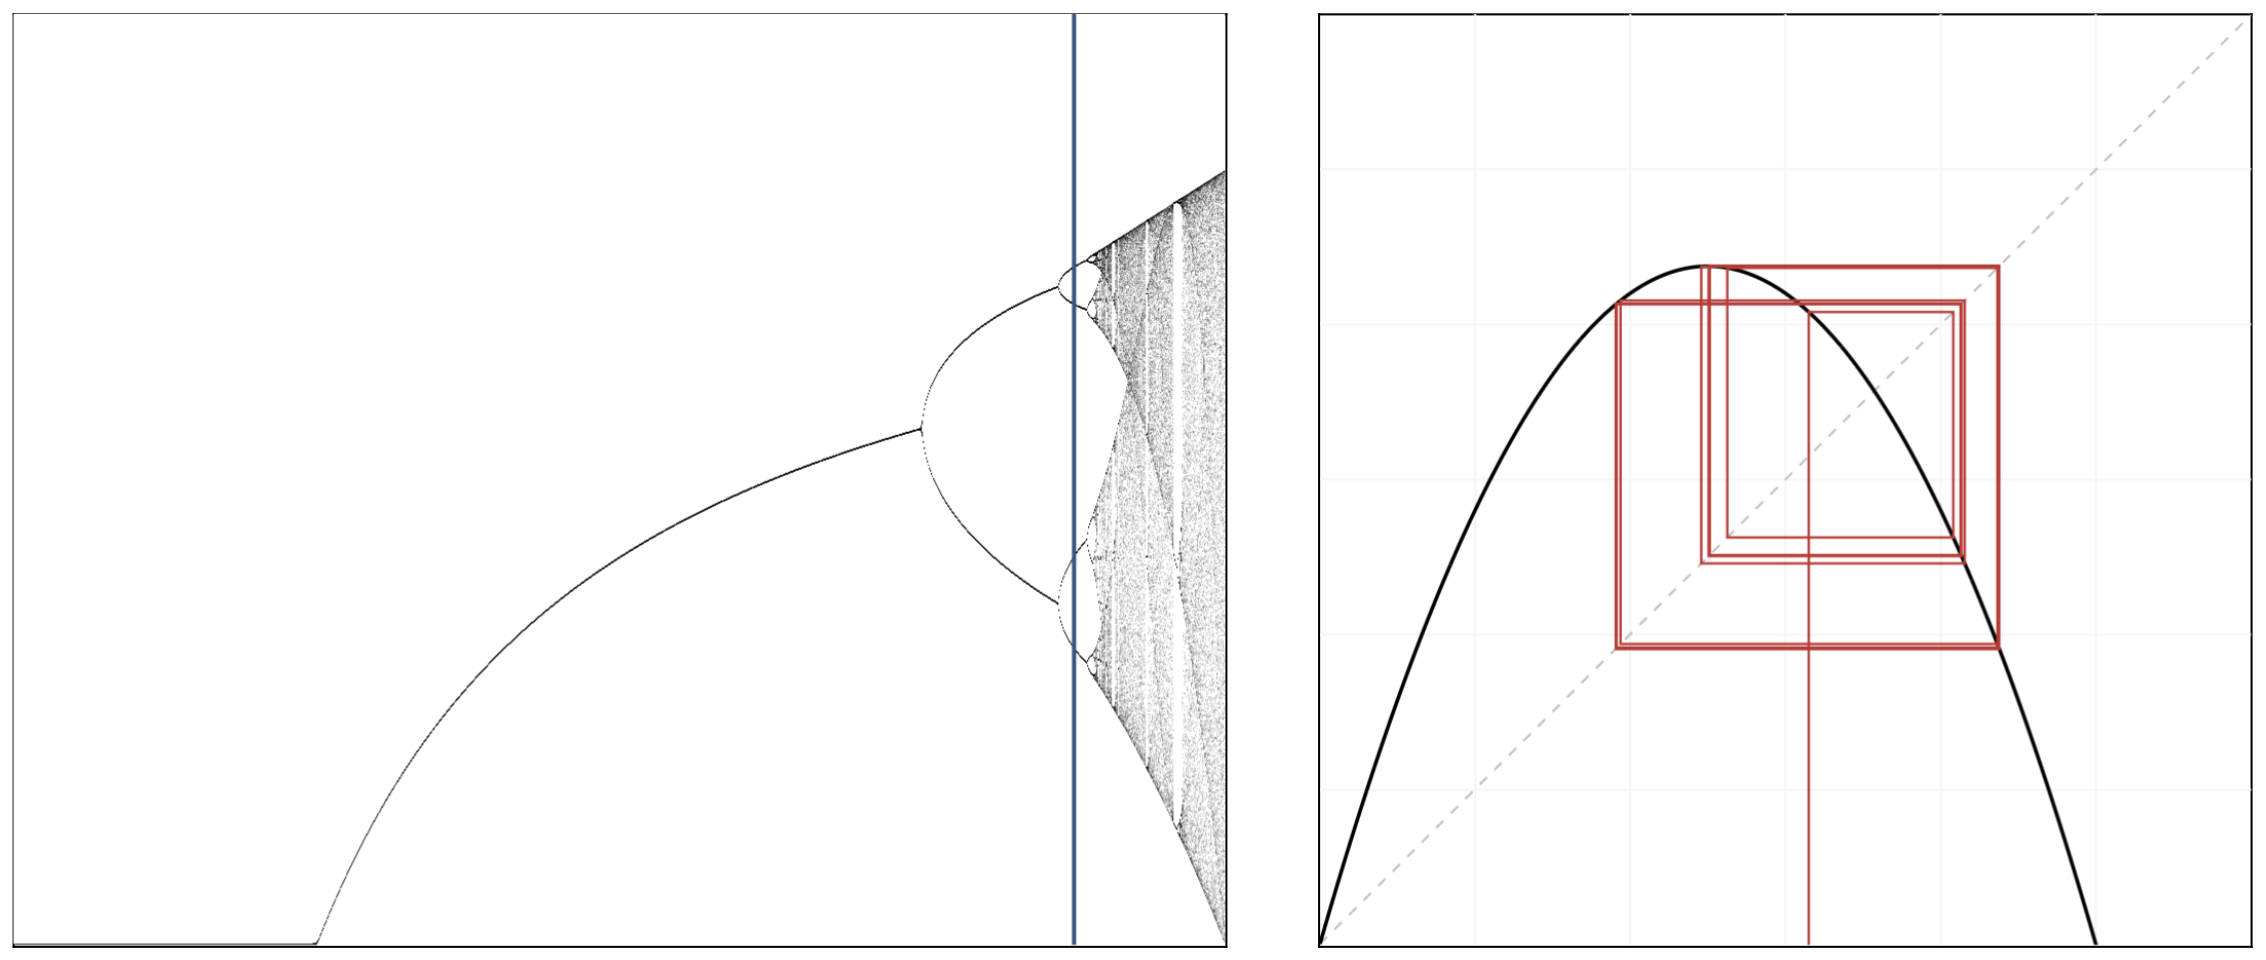
\includegraphics[width=0.86\textwidth]{figures/IMG_ch3/period_double.png}
    \caption{Bifurcation diagram of the logistic map $w\mapsto rw(1-w)$, showing the
    period doubling of stable states and the onset of chaos. The blue sample line on
    the left is at $r=3.5255$; the right-hand plot shows a trajectory of the map at
    the same $r$. The regime relevant to subcritical branching is $r=2p\in[0,1)$, off
    the left-hand edge of this diagram, where the dynamics are as simple as they can
    be.}
    \label{fig:period_double}
\end{figure}

In terms of $w$, \cref{eq:Ap-def} reads
\begin{equation}
\label{eq:Aw}
A(p) = \lim_{n\to\infty}\frac{S_n}{(2p)^n} = 2\lim_{n\to\infty}\frac{w_n}{r^n}.
\end{equation}
Now any sequence can be written as a telescoping product,
\begin{equation*}
x_n = x_0\lrb{\frac{x_1}{x_0}}\lrb{\frac{x_2}{x_1}}\cdots\lrb{\frac{x_n}{x_{n-1}}} = x_0\prod_{k=0}^{n-1}\frac{x_{k+1}}{x_k},
\qquad\text{so}\qquad
\lim_{n\to\infty}x_n = x_0\prod_{k=0}^{\infty}\frac{x_{k+1}}{x_k}.
\end{equation*}
Apply this with $x_n = w_n/r^n$. The ratio simplifies:
\begin{align*}
\frac{x_{k+1}}{x_k}
= \frac{w_{k+1}/r^{k+1}}{w_k/r^{k}}
= \frac{w_{k+1}}{w_k}\cdot\frac{1}{r}
= \frac{r w_k(1-w_k)}{w_k}\cdot\frac{1}{r}
= 1-w_k .
\end{align*}
Hence, with $x_0 = w_0 = \tfrac12$ and $A(p) = 2\lim_n x_n$,
\begin{equation*}
A(p) = 2\cdot\tfrac12\prod_{k=0}^{\infty}(1-w_k) = \prod_{k=0}^{\infty}(1-w_k),
\end{equation*}
and pulling out the $k=0$ factor, $1-w_0 = \tfrac12$,
\begin{equation}
\label{eq:prodFormula}
A(p) = \frac12\prod_{k=1}^{\infty}\lrb{1-w_k} = \frac12\prod_{k=1}^{\infty}\lrb{1-\frac{S_k}{2}}.
\end{equation}

\subsubsection*{Convergence}

For $0<w_k<1$ the infinite product $\prod_{k\ge1}(1-w_k)$ converges to a strictly
positive limit if and only if $\sum_{k\ge1}w_k<\infty$. From \cref{eq:logistic} with
$0<r<1$ and $0<w_n<1$ we have $w_{n+1}<rw_n$, so by induction $w_n\le w_0 r^n$. Since
$0<r<1$ this bound is summable, so $\sum_k w_k<\infty$ and the product converges to a
positive finite value. This also establishes what was asserted in \cref{sec:lateS}: the
limit \cref{eq:Ap-def} defining $A(p)$ exists and lies strictly between $0$ and
$\tfrac12$ for $p\in(0,\tfrac12)$.

\subsubsection*{Is this an advance?}

Only a modest one. \Cref{eq:prodFormula} is exact and its partial products are monotone
decreasing, so truncating gives a rigorous upper bound on $A(p)$ at every order --- which
the raw ratio $S_n/(2p)^n$ does not. But computing the factors still requires iterating
the nonlinear map to generate the $S_k$, so the near-critical difficulty is untouched.
What the product does supply is a route to the sharper result of the next subsection.

\subsection{An exact series and two-sided bounds}
\label{sec:Abounds}

The product can be converted into a telescoping sum, and the sum turns out to be much
more informative. Write $r=2p$ and note that the recursion factorises as
\begin{equation*}
S_{n+1} = rS_n\lrb{1-\frac{S_n}{2}} .
\end{equation*}
Define
\begin{equation*}
v_n = \frac{r^n}{S_n},
\end{equation*}
so that, by \cref{eq:Ap-def}, $v_n\to1/A(p)$. Then
\begin{equation*}
v_{n+1}-v_n
= \frac{r^{n+1}}{rS_n\lrb{1-\frac{S_n}{2}}} - \frac{r^n}{S_n}
= \frac{r^n}{S_n}\lrbs{\frac{1}{1-\frac{S_n}{2}}-1}
= \frac{r^n}{S_n}\cdot\frac{S_n/2}{1-\frac{S_n}{2}}
= \frac{r^n}{2-S_n}.
\end{equation*}
Summing from $v_0 = 1/S_0 = 1$ gives an exact representation of the quasi-stationary
mean.

\begin{proposition}[Series representation]
\label{prop:series}
For $p\in[0,\tfrac12)$, with $S_n$ generated by \cref{SnIter},
\begin{equation}
\label{eq:Aseries}
\frac{1}{A(p)} = 1 + \sum_{n=0}^{\infty}\frac{(2p)^n}{2-S_n}.
\end{equation}
\end{proposition}

\noindent
Unlike the product, this representation isolates the geometric decay in a factor that
does not depend on the dynamics at all; the whole of the nonlinearity sits in the
bounded denominator $2-S_n$. That is what makes it useful, because $S_n$ is confined to
$(0,1]$ and therefore $2-S_n$ is confined to $[1,2)$. Bounding the denominator by its
extremes and summing the resulting geometric series gives the following.

\begin{proposition}[Two-sided bounds]
\label{prop:bounds}
Write $\varepsilon = 1-2p$ for the distance from criticality. Then for
$p\in(0,\tfrac12)$
\begin{equation}
\label{eq:Abounds}
\frac{\varepsilon}{1+\varepsilon} \;<\; A(p) \;<\; \frac{2\varepsilon}{1+2\varepsilon},
\end{equation}
that is,
\begin{equation}
\label{eq:Aboundsexplicit}
\frac{1-2p}{2(1-p)} \;<\; A(p) \;<\; \frac{2(1-2p)}{3-4p}.
\end{equation}
The lower bound is exactly half the continuous-time constant of \cref{eq:Acts}:
\begin{equation}
\label{eq:halfAc}
A(p) > \tfrac12 A_{\text{c}}(p).
\end{equation}
\end{proposition}

\begin{proof}
Since $0<S_n\le1$ for all $n$, we have $1\le 2-S_n<2$ and hence
$\tfrac12 r^n < r^n/(2-S_n) \le r^n$, with the right-hand equality holding only at
$n=0$. Summing over $n\ge0$ and using $\sum_n r^n = 1/(1-r) = 1/\varepsilon$,
\begin{equation*}
1+\frac{1}{2\varepsilon} \;<\; \frac{1}{A(p)} \;<\; 1+\frac{1}{\varepsilon},
\end{equation*}
and inverting gives \cref{eq:Abounds}. Substituting $\varepsilon = 1-2p$ gives
\cref{eq:Aboundsexplicit}, whose lower bound is
$(1-2p)/\bigl(2(1-p)\bigr) = \tfrac12 A_{\text{c}}(p)$ by \cref{eq:Acts}.
\end{proof}

Two features of \cref{prop:bounds} deserve comment, because between them they account
for the whole shape of the discrete curve.

At the far subcritical end, $p\to0$, we have $\varepsilon\to1$ and the lower bound
tends to $\tfrac12$. Since $A(p)\le\tfrac12$ --- see \cref{prop:parity} below --- the
bound is asymptotically attained, and $A(0^+) = \tfrac12$. At the critical end,
$p\to\tfrac12^-$, we have $\varepsilon\to0$, the lower bound behaves like $\varepsilon$
and the upper like $2\varepsilon$; \cref{sec:asymptotic} shows that it is the upper
bound that is attained there. So $A(p)$ runs from its lower bound at one end of the
interval to its upper bound at the other, which is why no constant rescaling of
$A_{\text{c}}$ can reproduce it.

\begin{proposition}[Parity bound]
\label{prop:parity}
For the binary Galton--Watson process started from a single individual,
$A(p)\le\tfrac12$ for all $p\in[0,\tfrac12)$, with equality approached as $p\to0$.
\end{proposition}

\begin{proof}
Every individual leaves either $0$ or $2$ offspring, so $\zz_n$ is even for every
$n\ge1$. Conditional on survival we therefore have $\zz_n\ge2$, and hence
$\mean{\zz_n\mid \zz_n>0}\ge2$ for all $n\ge1$. Taking $n\to\infty$ and using
\cref{eq:qsmean}, $1/A(p)\ge2$. As $p\to0$ the conditional population is $2$ with
probability tending to one, so the bound is attained in the limit.
\end{proof}

\begin{table}[ht]
\centering
\caption{The constant $A(p)$ computed from the product \cref{eq:prodFormula} in
$60$-digit arithmetic, against the bounds of \cref{prop:bounds} and the near-critical
asymptotic $2(1-2p)$ of \cref{sec:asymptotic}. The bounds are loose in the middle of
the range and tighten at both ends: at $p=0.05$ the lower bound is already within
$3\%$ of $A$, whereas at $p=0.4999$ it is the upper bound that is within $0.1\%$.
The last two columns give the quasi-stationary mean and the number of factors of
\cref{eq:prodFormula} needed for the product to reach full precision --- the cost
that \cref{sec:practical} has to manage.}
\label{tab:Avals}
\begin{tabular}{ccccccr}
\toprule
$p$ & $\tfrac12 A_{\text{c}}(p)$ & $A(p)$ & $\dfrac{2(1-2p)}{3-4p}$ & $2(1-2p)$ & $1/A(p)$ & iterations\\
\midrule
0.05   & 0.473684 & 0.486180 & 0.642857 & 1.800000 & 2.0568 & 45 \\
0.1    & 0.444444 & 0.469382 & 0.615385 & 1.600000 & 2.1305 & 64 \\
0.2    & 0.375000 & 0.423895 & 0.545455 & 1.200000 & 2.3591 & 113 \\
0.3    & 0.285714 & 0.353967 & 0.444444 & 0.800000 & 2.8251 & 201 \\
0.4    & 0.166667 & 0.237647 & 0.285714 & 0.400000 & 4.2079 & 458 \\
0.45   & 0.090909 & 0.145069 & 0.166667 & 0.200000 & 6.8933 & 966 \\
0.48   & 0.038462 & 0.068011 & 0.074074 & 0.080000 & 14.7036 & 2\,473 \\
0.49   & 0.019608 & 0.036395 & 0.038462 & 0.040000 & 27.4764 & 4\,965 \\
0.499  & 0.001996 & 0.003944 & 0.003984 & 0.004000 & 253.519 & 48\,992 \\
0.4999 & 0.000200 & 0.000399 & 0.000400 & 0.000400 & 2504.65 & 478\,905 \\
\bottomrule
\end{tabular}
\end{table}

\subsection{Behaviour as \texorpdfstring{$p\to\tfrac12^-$}{p to 1/2}}
\label{sec:asymptotic}

The series \cref{eq:Aseries} also delivers the near-critical asymptotic, and does so
more transparently than the matching argument one is first tempted to try.

Fix $\varepsilon = 1-2p$ small. The summand $r^n/(2-S_n)$ involves two decays on very
different scales. The geometric factor $r^n = (1-\varepsilon)^n$ decays on the scale
$n\sim1/\varepsilon$, which is large. The survival probability $S_n$, by contrast, is
close to its critical behaviour $S_n\sim2/n$ over that whole range, and so has already
fallen to near zero after $O(1)$ generations. For the overwhelming majority of the terms
that carry weight, therefore, $S_n\approx0$ and the summand is $\approx r^n/2$. Summing,
\begin{equation*}
\sum_{n=0}^{\infty}\frac{r^n}{2-S_n} \;\approx\; \frac12\sum_{n=0}^{\infty}r^n = \frac{1}{2\varepsilon},
\end{equation*}
so $1/A(p)\sim 1/(2\varepsilon)$ and
\begin{equation}
\label{eq:Aasym}
\boxed{\;A(p) \sim 2\varepsilon = 2(1-2p)\qquad\text{as } p\to\tfrac12^-.\;}
\end{equation}
Equivalently $1/A(p)\sim 1/\bigl(2(1-2p)\bigr)$: the quasi-stationary mean diverges
like the reciprocal of the distance from criticality. In particular $A(p)$ meets the
axis at $p=\tfrac12$ with gradient $-4$, a fact used repeatedly below as a test of
candidate formulae.

The same result can be reached through the continuum equation of \cref{sec:riccati}.
With $\varepsilon = 1-2p$ the exact difference is
\begin{equation*}
S_{n+1}-S_n = (2p-1)S_n - pS_n^2 = -\varepsilon S_n - \tfrac12 S_n^2 + \tfrac{\varepsilon}{2}S_n^2 ,
\end{equation*}
and dropping the $O(\varepsilon S_n^2)$ term gives
$\dd S/\dd n = -\varepsilon S - \tfrac12 S^2$. Setting $u = 1/S$ linearises this to
$u' = \varepsilon u + \tfrac12$, with solution
\begin{equation*}
u(n) = C\ee^{\varepsilon n} - \frac{1}{2\varepsilon},
\qquad
S(n) = \frac{1}{C\ee^{\varepsilon n} - \frac{1}{2\varepsilon}} .
\end{equation*}
Matching $S_n\sim A\ee^{-\varepsilon n}$ for small $\varepsilon$ identifies $A = 1/C$,
and matching to the critical decay $S_n\sim2/n$ in the appropriate double limit fixes
$C\sim1/(2\varepsilon)$, recovering \cref{eq:Aasym}. The series argument is preferable
because it does not require the second matching step, which is the delicate one.

\begin{remark}[Rate of approach]
\label{rem:rate}
Numerically, $A(p)/2\varepsilon$ approaches $1$ rather slowly. Evaluating
\cref{eq:prodFormula} in high precision gives $A/2\varepsilon = 0.90987$, $0.98612$,
$0.99814$, $0.99977$ and $0.999972$ at $\varepsilon = 2\times10^{-2}$ down to
$2\times10^{-6}$. Fitting the deficit gives
$1 - A/2\varepsilon \approx \varepsilon\bigl(\ln(1/\varepsilon)+c\bigr)$ with
$c\approx0.78$, so
\begin{equation*}
A(p) = 2\varepsilon\Bigl[1+O\bigl(\varepsilon\ln(1/\varepsilon)\bigr)\Bigr].
\end{equation*}
The logarithmic correction is why \cref{eq:Aasym} is a good practical surrogate only
very close to criticality, and it is worth keeping in mind when \cref{sec:practical}
chooses the crossover point.
\end{remark}

\subsection{Why the discrete and continuous constants differ}
\label{sec:compare}

We can now settle the question raised by \cref{fig:dtct}. The two constants are
\begin{equation*}
A_{\text{c}}(p) = \frac{1-2p}{1-p}
\qquad\text{(continuous time)},
\qquad
A(p) = \lim_{n\to\infty}\frac{S_n}{(2p)^n}
\qquad\text{(discrete time)},
\end{equation*}
and the observation was that the first starts at $1$ where the second starts at
$\tfrac12$, yet halving the first does not superpose the curves.

\Cref{prop:bounds} explains this completely. What holds is not
$A = \tfrac12 A_{\text{c}}$ but the strict inequality $A > \tfrac12 A_{\text{c}}$, and
the inequality is attained only in the limit $p\to0$. Combining with
\cref{eq:Aasym,eq:Acts}, the ratio runs monotonically across the interval:
\begin{equation}
\label{eq:ratiolimits}
\frac{A(p)}{A_{\text{c}}(p)} \;\longrightarrow\; \tfrac12 \ \ (p\to0),
\qquad
\frac{A(p)}{A_{\text{c}}(p)} \;\longrightarrow\; 1 \ \ (p\to\tfrac12^-),
\end{equation}
taking the values $0.503$, $0.528$, $0.619$, $0.798$, $0.928$ and $0.988$ at
$p = 0.01,\,0.1,\,0.3,\,0.45,\,0.49,\,0.499$. No constant factor will do, because the
ratio is not constant.

The two endpoints have clean interpretations, and they are different in kind.

At $p\to0$ the factor of two is a counting effect. In the binary discrete model an
individual leaves either nothing or two offspring, so the surviving population is always
even (\cref{prop:parity}); deep in the subcritical regime, conditioning on survival means
conditioning on a population of exactly two, and the quasi-stationary mean is $2$. In
the continuous-time model a survivor is a single individual that simply has not yet died,
so the quasi-stationary mean is $1$. The reciprocals are $\tfrac12$ and $1$, and there is
the discrepancy.

At $p\to\tfrac12^-$ the factor disappears, because both constants are governed by the
same critical scaling. Expanding \cref{eq:Acts} near $p=\tfrac12$ gives
$A_{\text{c}}(p) = (1-2p)/(1-p) \to 2(1-2p)$, which is precisely \cref{eq:Aasym}. Near
criticality the discreteness of the generational clock stops mattering; what survives is
the universal $2\varepsilon$ behaviour, and the two models agree to leading order.

So the discrete curve is squeezed between $\tfrac12 A_{\text{c}}$ and its own critical
asymptote, hugging the former at one end and the latter at the other. That is the whole
content of \cref{fig:dtct}.

\subsection{Searching for a closed form}
\label{sec:GA}

Before the connection of \cref{sec:koenigs} was appreciated, a number of methods were
tried in the hope of an elementary formula for $A(p)$. Two are worth recording, partly
for the negative result and partly because the way they failed was itself informative.

The first was the continuum route already described in \cref{sec:riccati}: treat the map
as an ODE in the large-generation limit and solve it. This gives the shape of the decay
but, as noted there, leaves the constant of integration undetermined, which is to say it
leaves $A(p)$ undetermined.

The second was symbolic regression by genetic algorithm. The concept is simple: generate
fifty candidate functions at random, measure how closely each reproduces the target
curve, retain the best five, and build a fresh population of fifty by varying those five.
Measure again, and repeat the cycle of variation and selection many times over
\cite{stanley2002evolving,cohen2024physics}.

The first implementation searched a space of polynomials, partly on a hunch that the
answer might take that form and partly because such functions are simple to encode. In
the minimal case a genome is just a coefficient list $[a_0,\dots,a_k]$ for
\begin{equation*}
a_0 + a_1p + a_2p^2 + \cdots + a_kp^k
\end{equation*}
up to some chosen maximum order $k$, with the initial population drawn uniformly at
random. It quickly became apparent that many substantially different formulae produce
curves visually indistinguishable from the target --- but we wanted the exact one. On the
supposition that a true formula might have rational coefficients, a second version
searched
\begin{equation*}
\frac{a_0}{b_0} + \frac{a_1}{b_1}p + \cdots + \frac{a_k}{b_k}p^k,
\qquad [a_i],[b_i]\in\mathbb{Z}^{k+1},
\end{equation*}
and a third extended the space to ratios of two such polynomials, with genome in
$\mathbb{Z}^{4(k+1)}$. After numerous searches the best that emerged merely fitted the
high-precision numerical data well:
\begin{equation}
\label{eq:A1hat}
\hat A_1(p) = \frac{\tfrac12(1-2p)(1+2p)}{1 + \tfrac12 p - \tfrac52 p^2 - \tfrac65 p^3 + \tfrac65 p^4}.
\end{equation}
This passes through $(0,\tfrac12)$ and $(\tfrac12,0)$ and looks convincing to the eye,
but it fails the diagnostic of \cref{eq:Aasym}: differentiating at $p=\tfrac12$ gives a
gradient of $-2/0.55 = -3.636$ rather than the required $-4$.

Two years after this work was set aside it was revisited with more capable tooling,
using a symbolic tree search over progressively nested elementary functions of all
kinds. The conclusion was the same: many functions of widely varying form resemble the
target closely, and no satisfactory simple formula emerges even when solutions with
fewer components are explicitly favoured. Two arbitrary picks from the sea of similarly
performing candidates:
\begin{multline}
\label{eq:A2hat}
\hat A_2(p) = 0.31696448624690005\,
\ln\!\Biggl(\Biggl|\cos\!\biggl(\left(\frac{1}{3.19801133824532}\right)^{\!1/4}\\
+\, p\biggl[\sin\!\Bigl(\cos\!\bigl(|p|\,(0.621865696665606 - p)\,\cos(\ee^{\ee^{p}})\bigr)\Bigr) + |p|\biggr]\biggr)\Biggr|\Biggr)
+ 0.5982282661889831
\end{multline}
and, more concisely,
\begin{equation}
\label{eq:A3hat}
\hat A_3(p) = \frac{-0.616647881739505\,\ee^{-0.552605335919693\,\ee^{p}}}{\sin(\cos p) - |p|} + 0.921964323679771 .
\end{equation}
\Cref{eq:A2hat} is quoted after removing redundancies such as a factor $p/p$ that the
program had introduced --- neutral mutations, in effect, carrying no fitness cost and so
never selected against.

\begin{figure}[ht]
\centering
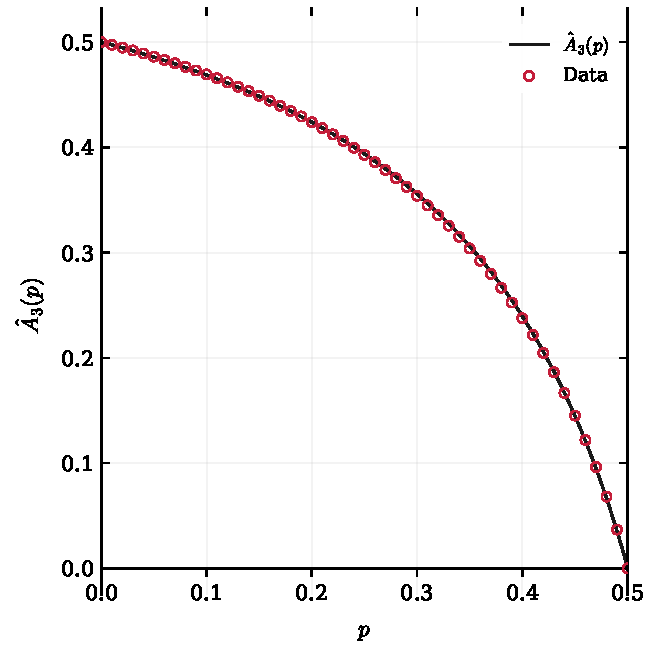
\includegraphics[width=0.56\textwidth]{figures/IMG_ch3/A3_hat_plot.pdf}
\caption{The symbolic-regression candidate $\hat A_3(p)$ of \cref{eq:A3hat} (solid)
against numerically computed values of $A(p)$ (red circles). The agreement is
excellent to the eye across the whole interval, which is exactly the problem: the fit
is not evidence of correctness. $\hat A_3$ misses the critical point by
$\hat A_3(\tfrac12)=9.1\times10^{-4}$ rather than $0$, and arrives there with gradient
$-3.63$ instead of $-4$. Errors of this size are invisible here but are fatal for
$1/A$ near criticality.}
\label{fig:A3hat}
\end{figure}

The recurring defect is the same in every case. The candidates either fail to pass
through $(\tfrac12,0)$ or fail to arrive there with gradient $-4$, and near criticality
this matters enormously: as $A\to0$, an error in $A$ of vanishing absolute size produces
an $O(1)$ --- eventually unbounded --- error in the quasi-stationary mean $1/A$. A
formula can look perfect on a plot of $A$ and be useless on a plot of $1/A$.

A pragmatic patch is to splice the asymptotic onto a fitted curve, as in
\begin{equation}
\label{eq:A4hat}
\hat A_4(p) =
\begin{cases}
-0.04011483983619545\,\ee^{\ee^{2p}} + 0.6079994336528085, & p < 0.499962,\\[2mm]
2-4p, & p \ge 0.499962,
\end{cases}
\end{equation}
which does work. But if one is going to splice, it is better to splice onto something
exact, and \cref{sec:practical} does so.

The deeper lesson from these searches is worth stating plainly, because it points
directly at the next subsection. That an enormous number of very different formulae can
behave almost identically over a bounded interval is not merely an inconvenience of the
method; it is a symptom. Curve-fitting cannot distinguish a function that has a closed
form from one that does not.

\subsection{The Koenigs connection}
\label{sec:koenigs}

It was only some time after the search had been abandoned that a dynamical argument
emerged explaining why no elementary closed form should be expected. In short, $A(p)$
is a value of the Koenigs linearising function of the logistic map, and that function is
known to be non-elementary throughout the parameter range we need.

\begin{definition}[Koenigs function]
\label{def:koenigs}
Let $f(z) = rz(1-z)$ have a fixed point at $z=0$ with multiplier $r = f'(0)$, and
suppose $|r|\notin\{0,1\}$. Koenigs \cite{Koenigs1884} proved that there exists a unique
function $\psi_r$, analytic near the origin, satisfying the Schr\"oder equation
\begin{equation}
\label{eq:schroder}
\psi_r\bigl(f(z)\bigr) = r\,\psi_r(z),
\qquad
\psi_r(0)=0,
\qquad
\psi_r'(0)=1 .
\end{equation}
\end{definition}

\noindent
The Koenigs function is a change of coordinate that straightens the dynamics: in the
$\psi$ coordinate the nonlinear map $f$ becomes multiplication by $r$
(\cref{fig:koenigs}). In our case $f(z)=rz(1-z)$ is exactly \cref{eq:logistic}, with
$z = w_n$ and $f(z) = w_{n+1}$, and the multiplier is $r = 2p\in(0,1)$ --- an attracting
fixed point, which is the classical Koenigs setting.

\begin{figure}[ht]
\centering
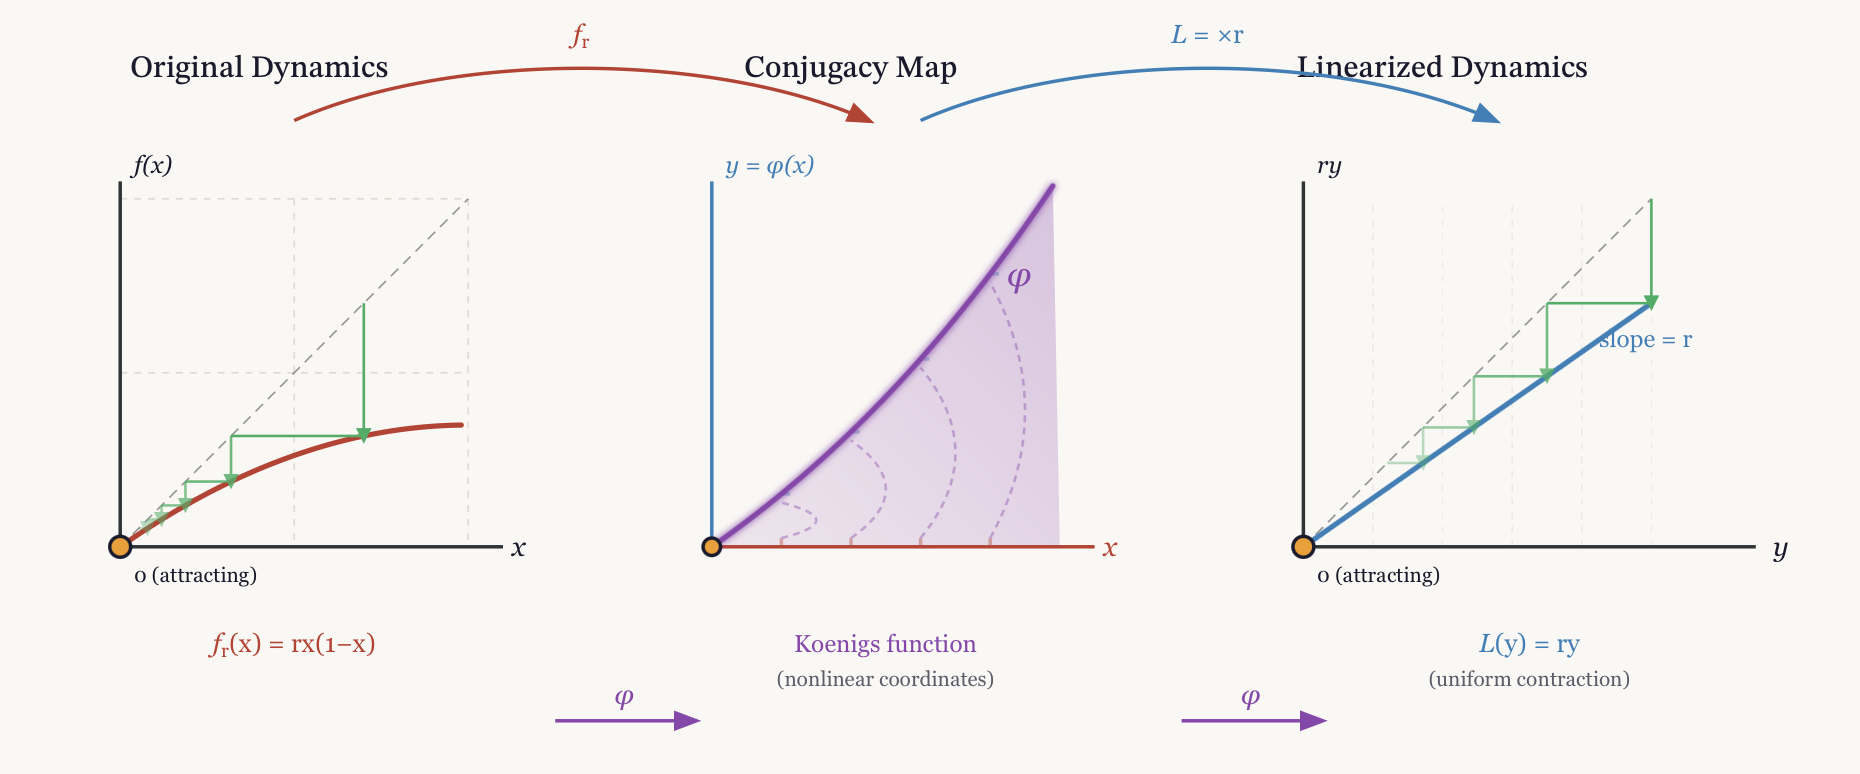
\includegraphics[width=0.72\textwidth]{figures/IMG_ch3/figure2_koenigs_linearization.png}
\caption{Koenigs linearisation of the logistic map near an attracting fixed point.
The nonlinear dynamics $x\mapsto f_r(x) = rx(1-x)$ are conjugated by $\psi_r$ to the
linear map $y\mapsto ry$; the diagram displays the functional relation
$\psi_r(f_r(x)) = r\psi_r(x)$ and the role of $\psi_r$ as the coordinate change that
straightens the dynamics.}
\label{fig:koenigs}
\end{figure}

\begin{proposition}
\label{prop:AisKoenigs}
For $p\in(0,\tfrac12)$ and $r=2p$,
\begin{equation}
\label{eq:AeqKoenigs}
A(p) = 2\,\psi_r\!\lrb{\tfrac12}.
\end{equation}
\end{proposition}

\begin{proof}
Iterating \cref{eq:schroder} along the orbit $w_0,w_1,w_2,\dots$ of \cref{eq:logistic}
gives $\psi(w_1) = r\psi(w_0)$, hence $\psi(w_0)=\psi(w_1)/r$; similarly
$\psi(w_1)=\psi(w_2)/r$, so $\psi(w_0)=\psi(w_2)/r^2$; and by induction
\begin{equation}
\label{eq:induction}
\psi(w_0) = \frac{\psi(w_n)}{r^n}\qquad\text{for every }n .
\end{equation}
Since \cref{eq:induction} holds for all $n$ we may pass to the limit,
\begin{equation*}
\psi(w_0) = \lim_{n\to\infty}\frac{\psi(w_n)}{r^n}.
\end{equation*}
Now the normalisation $\psi(0)=0$, $\psi'(0)=1$ means $\psi(z)/z\to1$ as $z\to0$, and
$w_n = S_n/2\to0$ because $r<1$. Replacing $\psi(w_n)$ by $w_n$ in the limit is therefore
legitimate, and
\begin{equation*}
\psi(w_0) = \lim_{n\to\infty}\frac{w_n}{r^n}.
\end{equation*}
Comparing with \cref{eq:Aw} and using $w_0 = S_0/2 = \tfrac12$ gives
$A(p) = 2\psi_r(\tfrac12)$.
\end{proof}

\subsubsection*{When is \texorpdfstring{$\psi_r$}{psi} elementary?}

The answer is: essentially never. The logistic family is affinely conjugate to the
canonical quadratic family $P_c(z) = z^2+c$; substituting $x = -z/r + \tfrac12$ in
$f_r$ gives $P_c$ with
\begin{equation}
\label{eq:cofr}
c = \frac{2r-r^2}{4}.
\end{equation}
Under \cref{eq:cofr} the interval $r\in(0,1)$ maps to $c\in(0,\tfrac14)$
(\cref{fig:conjugacy}). The relevance of this is a rigidity theorem of Becker and
Bergweiler \cite{Becker1995}: for a rational map $R$ of degree at least two with a fixed
point of multiplier $\lambda$, $0<|\lambda|<1$, the associated Koenigs linearisation
satisfies an algebraic differential equation only when $R$ is analytically conjugate to
a monomial map $z\mapsto z^{\pm d}$ or to a Chebyshev polynomial $\pm T_d$. For the
quadratic family these exceptional cases are exactly $c=0$ and $c=-2$, corresponding
under \cref{eq:cofr} to $r=2$ and $r=4$ respectively.

Since every elementary function in the sense of Liouville --- algebraic functions,
exponentials, logarithms and their finite combinations --- satisfies an algebraic
differential equation, a function that satisfies none (a hypertranscendental function)
cannot be elementary. And
\begin{equation*}
\lrb{0,\tfrac14}\cap\{0,-2\} = \emptyset,
\end{equation*}
so no $r$ in our range is exceptional: for each fixed $r\in(0,1)$, the Koenigs function
$\psi_r$ is hypertranscendental, and in particular not elementary.

\begin{figure}[ht]
\centering
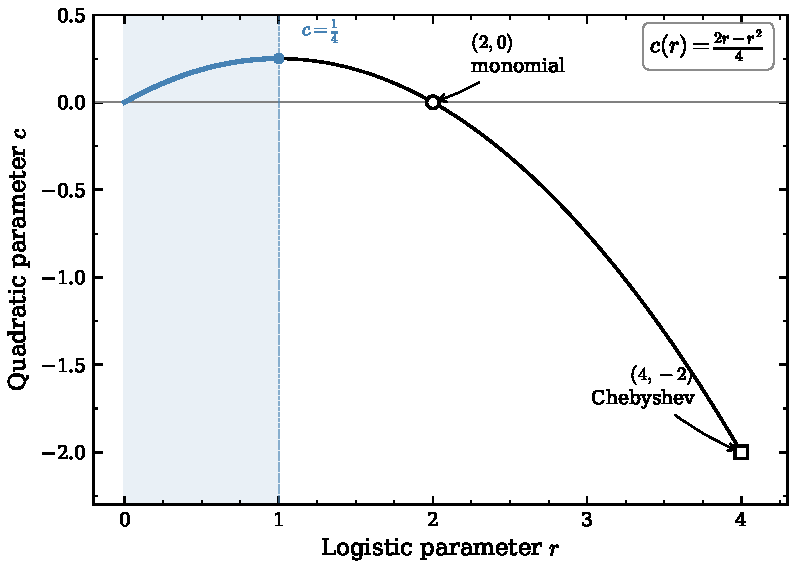
\includegraphics[width=0.66\textwidth]{figures/IMG_ch3/figure1_parameter_conjugacy.pdf}
\caption{The affine parameter correspondence $c(r) = (2r-r^2)/4$ between the logistic
family $f_r(x)=rx(1-x)$ and the quadratic family $P_c(z)=z^2+c$. The shaded segment is
$r\in(0,1)$, the subcritical branching window, which maps to $c\in(0,\tfrac14)$. The
two integrable parameters, $r=2$ ($c=0$, monomial) and $r=4$ ($c=-2$, Chebyshev), lie
outside it.}
\label{fig:conjugacy}
\end{figure}

The two exceptional parameters are worth writing out, both as a check on the machinery
and because they show just how special the solvable cases are.

\paragraph{The monomial case, $r=2$.}
Here $f_2(x) = 2x(1-x)$. The substitution $u = 1-2x$ gives
\begin{equation*}
u_{n+1} = 1 - 2\bigl(2x_n(1-x_n)\bigr) = 1-4x_n+4x_n^2 = (1-2x_n)^2 = u_n^2 ,
\end{equation*}
and the map $u\mapsto u^2$ is linearised by the logarithm, since
$\ln(u^2) = 2\ln u$. Returning to $x$ and imposing the normalisation of
\cref{def:koenigs},
\begin{equation}
\label{eq:psi2}
\psi_2(x) = -\tfrac12\ln(1-2x),
\end{equation}
which is readily verified:
$\psi_2(f_2(x)) = -\tfrac12\ln\bigl((1-2x)^2\bigr) = 2\bigl[-\tfrac12\ln(1-2x)\bigr] = 2\psi_2(x)$.

\paragraph{The Chebyshev case, $r=4$.}
Here $f_4(x) = 4x(1-x)$ is conjugate to $T_2(z) = 2z^2-1$ by a trigonometric
substitution. Putting $x = \sin^2\theta$,
\begin{equation*}
f_4(x) = 4\sin^2\theta\cos^2\theta = (2\sin\theta\cos\theta)^2 = \sin^2(2\theta),
\end{equation*}
so the map is a doubling $\theta\mapsto2\theta$ in the $\theta$ coordinate. The
multiplier at the origin is $4$, not $2$, which suggests that the linearisation involves
$\theta^2$; and indeed
\begin{equation}
\label{eq:psi4}
\psi_4(x) = \bigl(\arcsin\sqrt{x}\,\bigr)^2 .
\end{equation}
Using $\arcsin(2u\sqrt{1-u^2}) = 2\arcsin u$ with $u=\sqrt{x}$,
$\psi_4(f_4(x)) = (2\arcsin\sqrt{x})^2 = 4\psi_4(x)$; and as $x\to0$,
$\arcsin\sqrt{x}\approx\sqrt{x}$, so $\psi_4(x)\approx x$ and $\psi_4'(0)=1$.

\begin{remark}[Attracting versus repelling]
\label{rem:attractrepel}
At $r=2$ and $r=4$ the multiplier at the origin is $|r|>1$, so the origin is repelling.
The functions \cref{eq:psi2,eq:psi4} are therefore Poincar\'e-type linearisations rather
than attracting-Koenigs maps, and neither parameter lies in the branching window
$r=2p\in[0,1)$ in any case. They are recorded here to show what a solvable case looks
like, not because they bear on $A(p)$.
\end{remark}

\subsubsection*{What this does and does not establish}

It is important to be precise about the status of the conclusion, because it is easy to
overstate.

What is established is that for each fixed $r\in(0,1)$ the function $z\mapsto\psi_r(z)$
is hypertranscendental. Combined with \cref{prop:AisKoenigs}, this says that $A(p)$ is a
value of a non-elementary function, evaluated at the fixed point $z=\tfrac12$, for every
$p$ in the subcritical range. It is a strong indication that the search of \cref{sec:GA}
was doomed, and it explains the phenomenology of that search: the object being fitted is
defined only by the dynamics that generate it.

What is not established is that the map $p\mapsto A(p)$ admits no elementary description.
Hypertranscendence of $\psi_r$ in its argument $z$ is a statement about one variable;
$A(p) = 2\psi_{2p}(\tfrac12)$ varies the parameter and freezes the argument, and the two
questions are logically distinct. A rigorous negative result for $p\mapsto A(p)$ would
require a transcendence statement about the values, not the functions, and none is
claimed here. The honest summary is that no closed form is known, that the structural
reason for expecting none is the one just given, and that the numerical evidence of
\cref{sec:GA} is entirely consistent with there being none.

It is worth seeing where in the quadratic family our parameters sit, because the picture
makes the difficulty look structural rather than accidental. The main cardioid of the
Mandelbrot set --- the set of $c$ for which $z^2+c$ has an attracting fixed point --- is
parametrised by that point's multiplier $\lambda$ through $c = \lambda/2 - \lambda^2/4$,
which is exactly \cref{eq:cofr} with $\lambda = r$. The branching window $r\in(0,1)$ is
therefore the real diameter of the main cardioid, traversed from the centre $c=0$ out to
the parabolic cusp $c=\tfrac14$, where $\lambda=1$ and the process turns critical.
\Cref{fig:mandelbrot} places the segment in context; the two integrable parameters $c=0$
and $c=-2$ are marked, and the open window contains neither.

Throughout the window the Julia set is a quasicircle bounding the basin of the
attracting fixed point, and it is a genuine fractal for every $c$ in the interval. The
Koenigs function is the conformal coordinate that linearises the dynamics inside that
basin, so its natural domain is bounded by exactly this curve. A function whose domain
of definition has no smooth description is not a promising candidate for a closed form,
and $A(p)$, being one of its values, inherits the difficulty. The contrast with the
integrable cases is sharp: at $c=0$ the Julia set degenerates to the unit circle, and it
is precisely there that the linearisation becomes elementary, \cref{eq:psi2}.

\begin{figure}[ht]
\centering
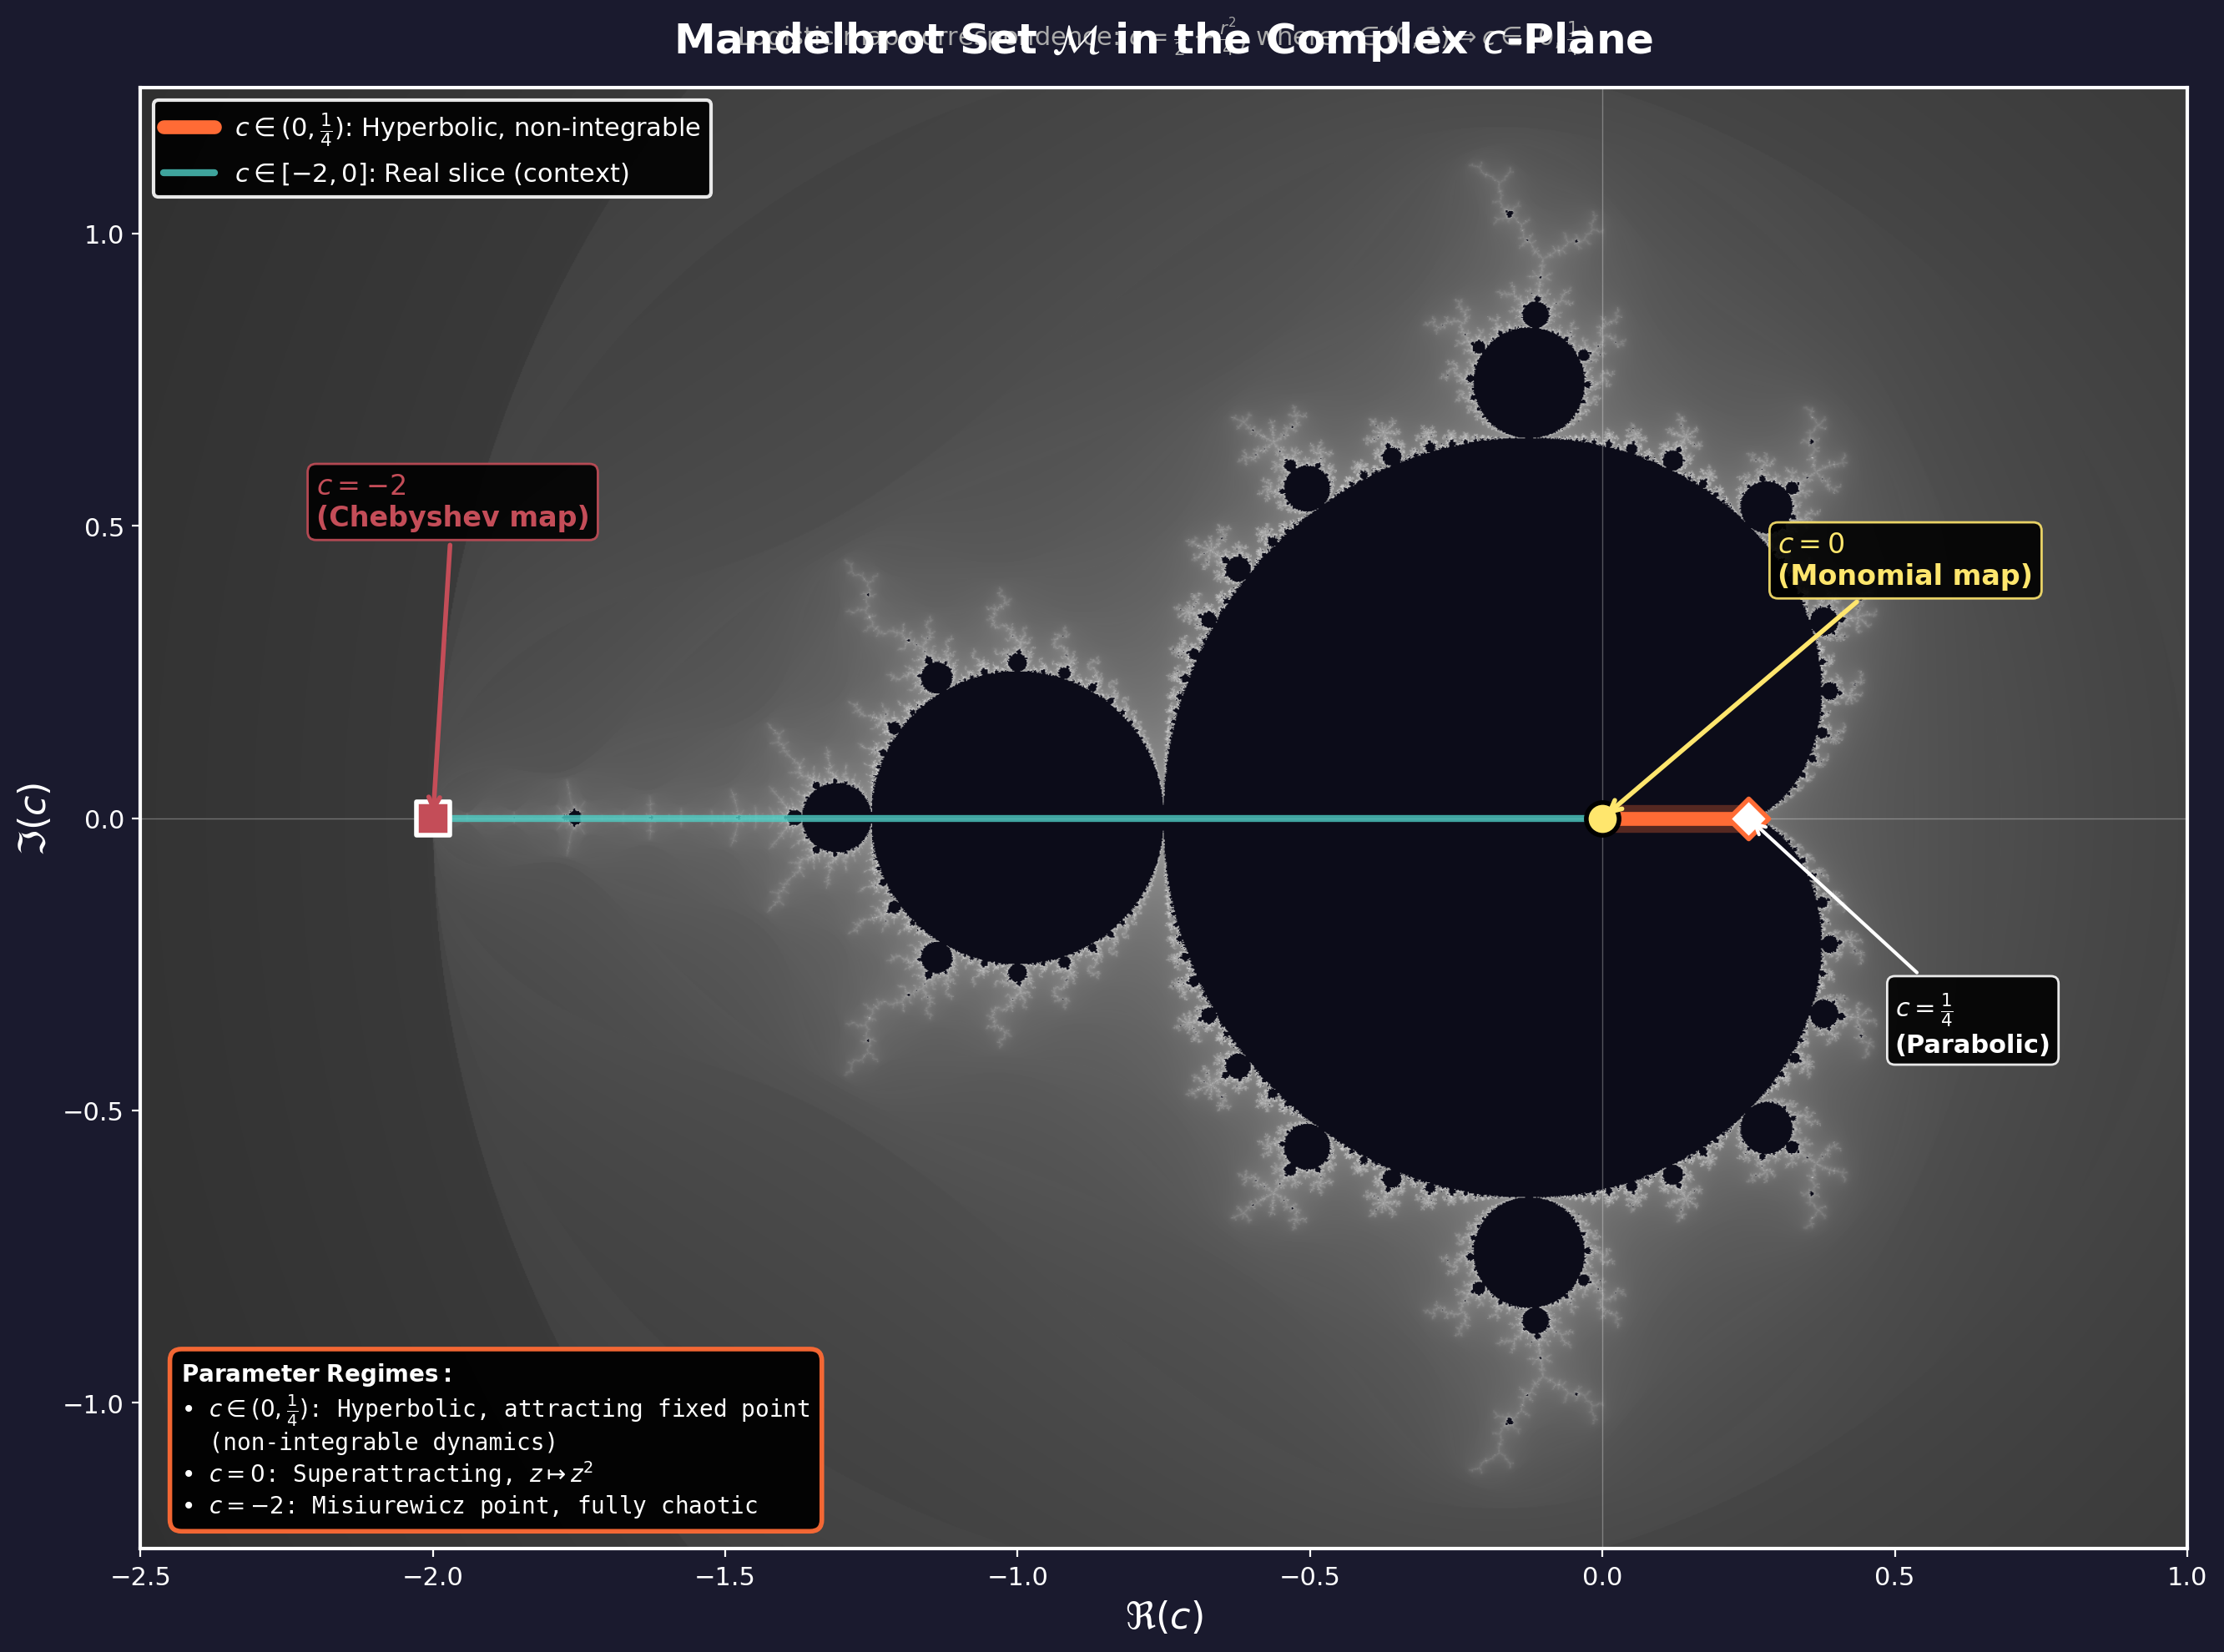
\includegraphics[width=0.92\textwidth]{figures/IMG_ch3/figure4_mandelbrot_context.png}
\caption{The Mandelbrot set in the complex $c$-plane, with the interval
$c\in(0,\tfrac14)$ highlighted. Under the correspondence $c=(2r-r^2)/4$ of
\cref{eq:cofr} this is the image of the subcritical branching window $r=2p\in(0,1)$,
and it forms the real diameter of the main cardioid, running from the centre $c=0$ to
the parabolic cusp $c=\tfrac14$ --- which is criticality. The two integrable
parameters are marked: $c=0$ (monomial, reached in logistic coordinates at $r=2$) and
$c=-2$ (Chebyshev, $r=4$), the latter at the far tip of the real slice. Note that
$c(r)=c(2-r)$, so each $c\in(0,\tfrac14)$ is the image of two logistic parameters,
$r$ and $2-r$; these correspond to the two fixed points of $z^2+c$, with multipliers
$r$ and $2-r$, and it is the attracting one, $r<1$, that governs $A(p)$.}
\label{fig:mandelbrot}
\end{figure}

\subsection{Computing \texorpdfstring{$A(p)$}{A(p)} in practice}
\label{sec:practical}

In the absence of an exact formula we are left with approximation, and the two regimes
of \cref{sec:Abounds} suggest how to split the work.

Over most of the interval, direct iteration is entirely satisfactory: the infinite
product \cref{eq:prodFormula} converges quickly, its partial products bound $A(p)$ from
above at every order, and modest numbers of iterations give many digits. The difficulty
is confined to a neighbourhood of $p=\tfrac12$, and it has two parts. First, as
$A(p)\to0$ the quantity of interest $1/A$ diverges, so a fixed absolute error in $A$
becomes an unbounded error in the quasi-stationary mean. Second --- and this is the
binding constraint --- as the process is defined ever closer to criticality its
lifetime, though still finite, grows enormously, and $S_n$ recedes to zero ever more
slowly. The iteration must be carried to a generation at which $S_n$ is essentially
unchanging, and \cref{tab:Avals} shows what that costs: about $10^2$ iterations at
$p=0.2$, $10^3$ at $p=0.45$, but nearly $5\times10^5$ at $p=0.4999$.

The remedy is to hand the near-critical region to the asymptotic \cref{eq:Aasym}, which
is exact in the limit and cheap everywhere. This gives
\begin{equation}
\label{eq:Apractical}
A(p) \approx
\begin{cases}
\displaystyle \frac12\prod_{k=1}^{N}\lrb{1-\frac{S_k}{2}}, & p<c,\quad N\gg1,\\[14pt]
2-4p, & p\ge c,
\end{cases}
\end{equation}
with the crossover $c$ chosen just below $\tfrac12$. \Cref{rem:rate} indicates where to
put it: the relative error of the asymptotic is about $\varepsilon\ln(1/\varepsilon)$, so
at $c = 0.4999$ ($\varepsilon = 2\times10^{-4}$) the asymptotic is already accurate to
about two parts in $10^3$, while the product still converges in a few hundred thousand
iterations. Any $c$ in the range $0.499$--$0.4999$ gives a scheme accurate to better than
one per cent throughout, and the two branches can be blended over a narrow window if
continuity of the derivative matters.

This is the recipe used for the numerical values quoted throughout this chapter,
including those in \cref{fig:condmean,tab:Avals}.

\FloatBarrier
